\documentclass{beamer}

\usepackage{beamerthemesplit} 
\usetheme{Frankfurt}
\usecolortheme{whale}
\setbeamerfont{professionalfonts}{family=\rm}
\title{Image Stitching}
\author[\textbf{HHSST}]{\textbf{cs482}\\
Travis Hile\\
Jeremiah Howdeshell\\
Chris Sahno\\
Kevin St.Andrie\\
Martin Taheri
}



\date{\today}

\begin{document}

\frame{\titlepage}

\section[Outline]{}
\frame{\tableofcontents}

\section{Objective}
\subsection{Investigate Image Stitching}
\frame
{
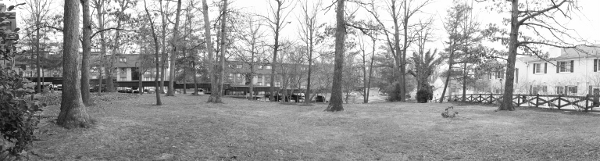
\includegraphics[scale=.5]{rptImages/panoramic_shot.jpg}
\begin{itemize}
\item Investigate and understand the methods used to develop panoramic and composite images (such as the one above)
\item Adapt these techniques into a portable code library which could conceivably be run on a smartphone (such as an Android device).
\end{itemize}
}
\section{Methodology}
\frame
{
\begin{itemize}
	\item To that end, using a tripod and a digital camera, we collected 96 images of George Mason University's campus.
	\item We then built a routine to stitch images together, using this dataset of images to test the output.
\end{itemize}
}

\subsection{Dataset Collection}
\frame
{
 	\frametitle{Rotational Panorama Images}
	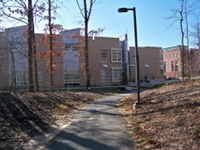
\includegraphics[scale =.5]{rptImages/100_2992.jpg}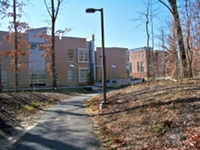
\includegraphics[scale =.5]{rptImages/100_2993.jpg}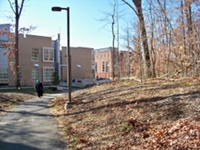
\includegraphics[scale =.5]{rptImages/100_2994.jpg}\\
	40 images were taken at $10^{\circ}$ increments from the same fixed position along the path between the Research building and the Arts building.
}

\frame
{
 	\frametitle{Engineering Parallax}
	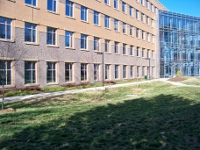
\includegraphics[scale =.5]{rptImages/100_3038.jpg}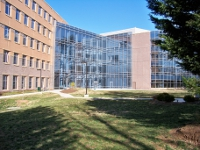
\includegraphics[scale =.5]{rptImages/100_3042.jpg}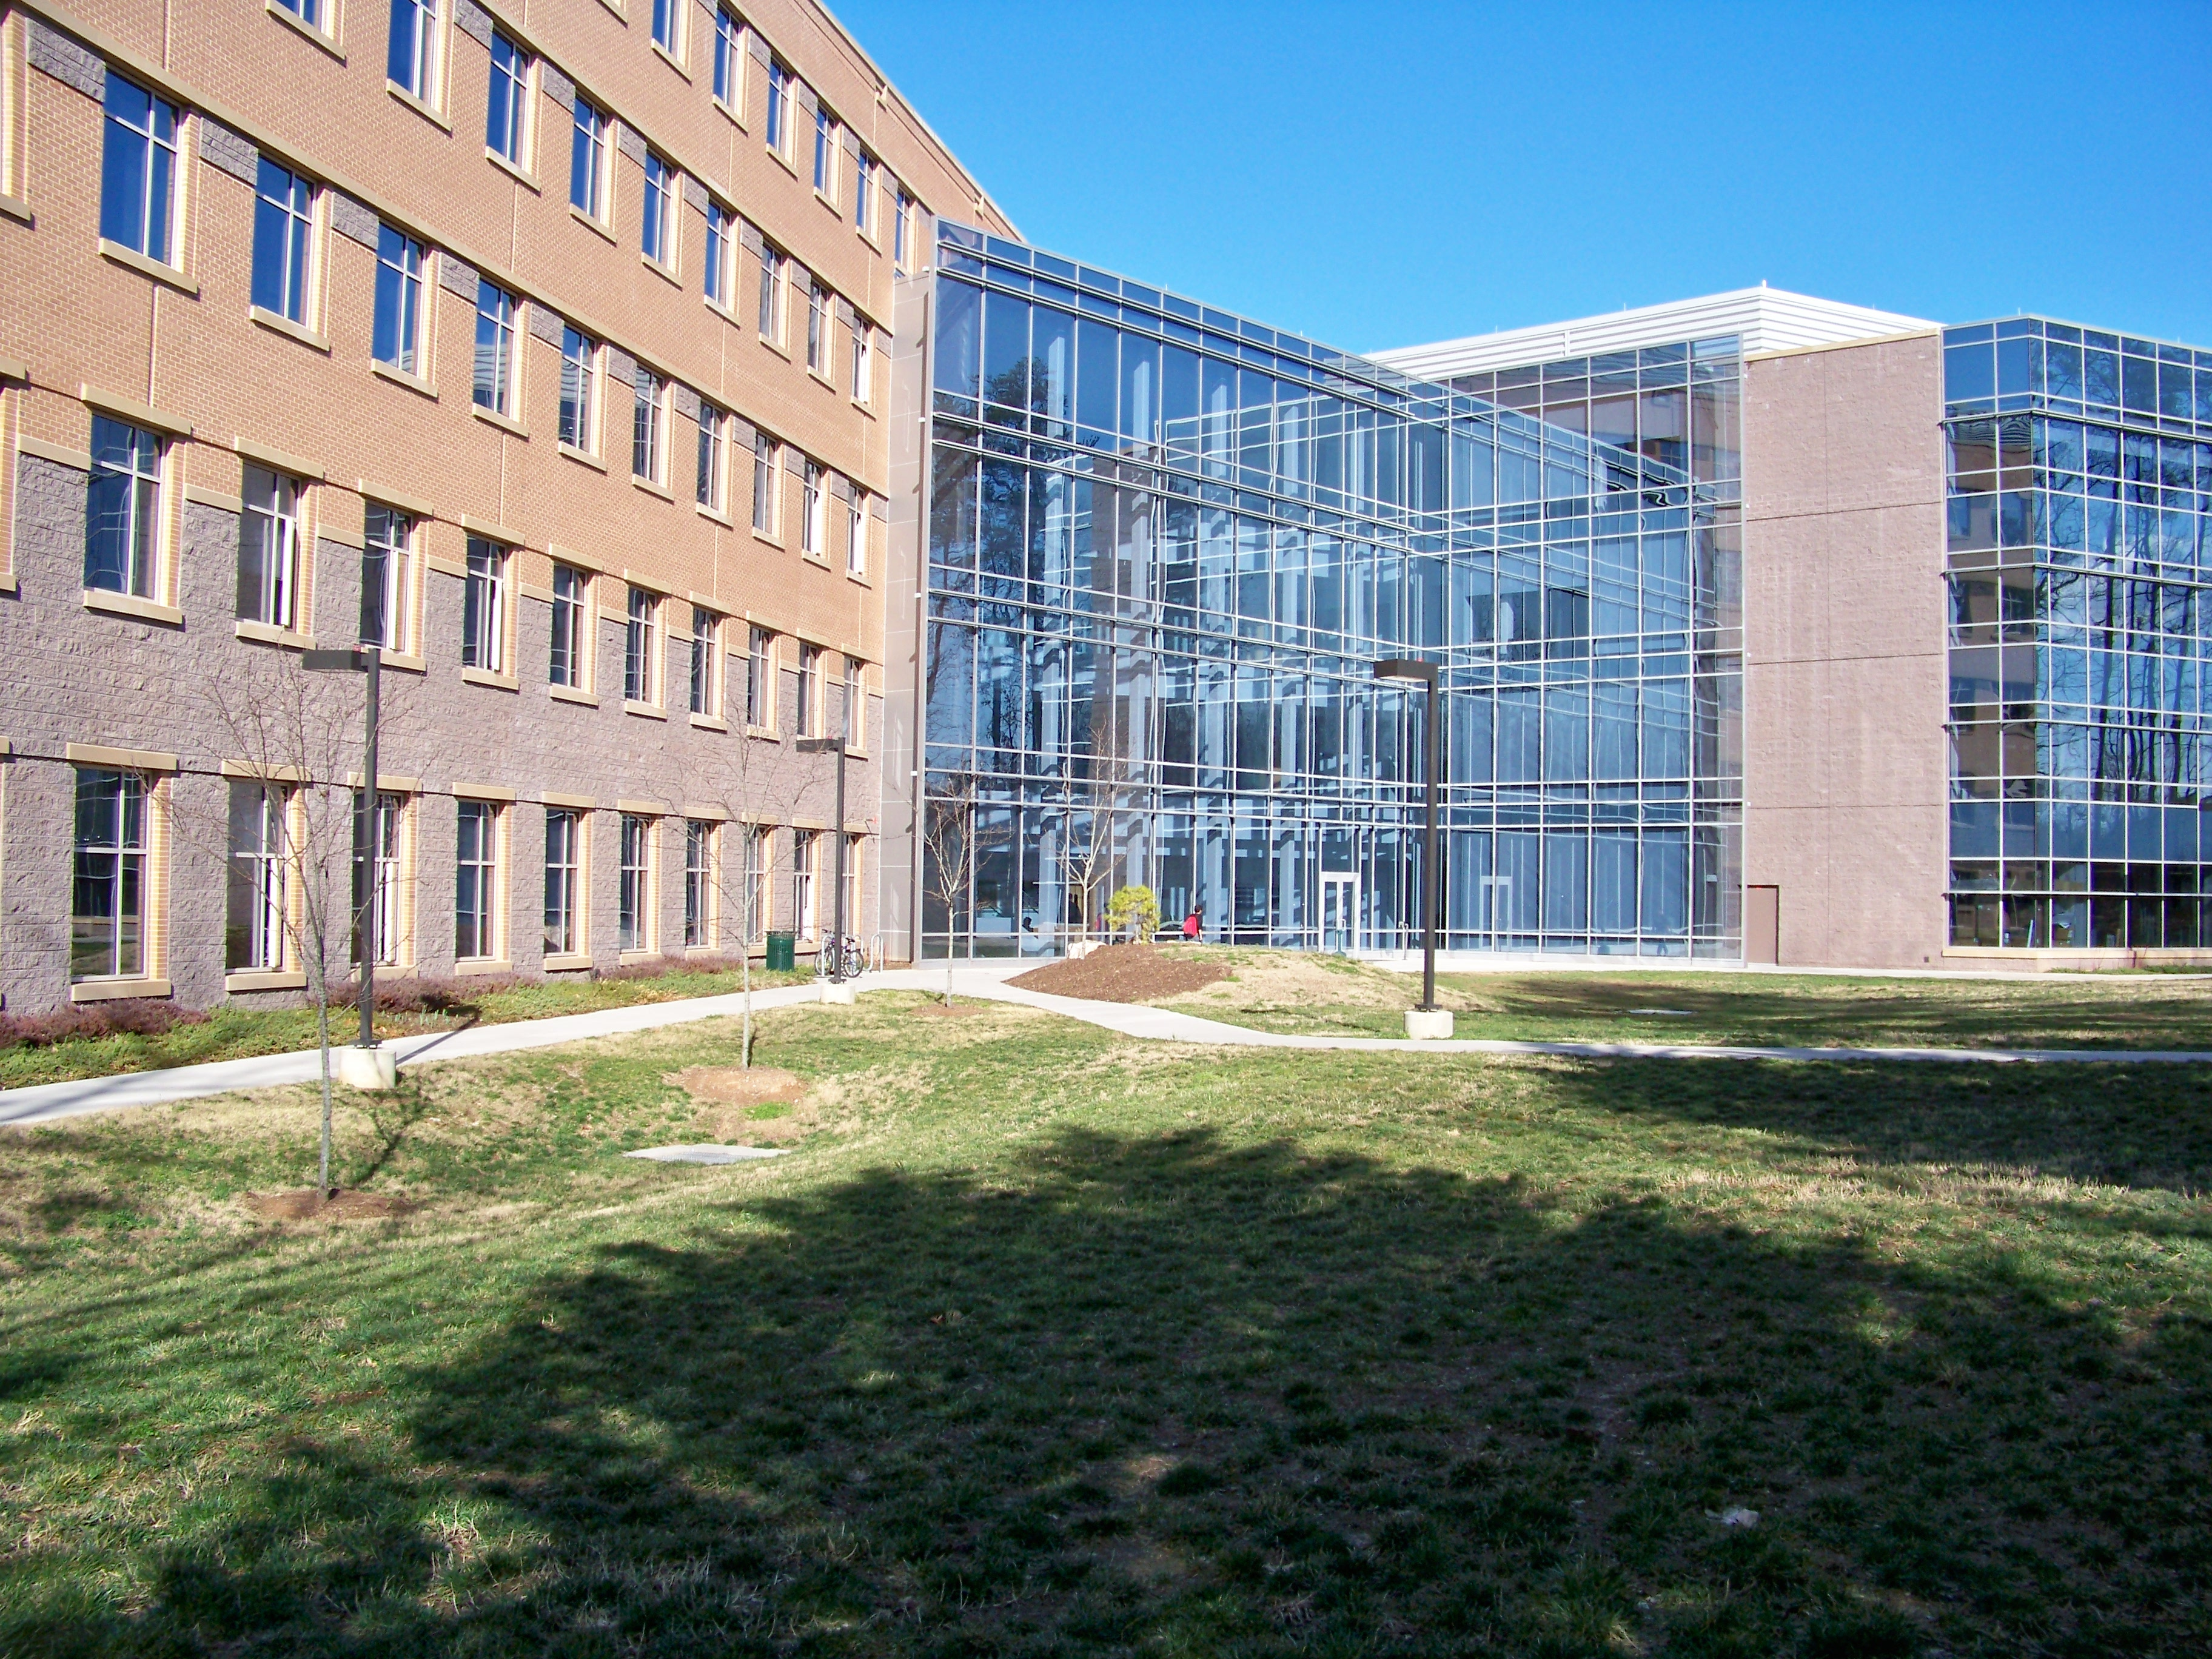
\includegraphics[scale =.5]{rptImages/100_3047.jpg}\\
	27 images were taken of the Engineering building from different vantage points, in order to generate parallax errors issues.
}
\section{Stitching Process}
\subsection{The General Idea}
\frame {
 	\frametitle{The Image Stitching Process}
\begin{enumerate}
\item Take two images, A \& B
\item Find keypoints for each image using SURF
\item For each keypoint in A, find closest match in B and pair up
\item Build a `homography' for the two images using RANSAC
\item Warp image B using the homography and paste onto image A
\end{enumerate}
}

\subsection{Our Implementation}
\frame {
	\frametitle{Computer Vision Libraries to Speed Things Up}
	\begin{itemize}
		\item Python \& OpenCV
			\begin{itemize}
				\item Built an OpenCV based program in using Python as a proof of concept
				\item Used the SURF and RANSAC routines in the OpenCV library
				\item Nearest neighbor implemented in Python (very slow!)
			\end{itemize}
		\item Android \& Boofcv
			\begin{itemize}
				\item Built an Android application for everyday use
				\item Again, used routines in the library
				\item Due to memory and speed issues, best for small images ( $\leq 640x480 $)
			\end{itemize}		
	\end{itemize}
}
\end{document}
